\documentclass{beamer}
\usetheme{metropolis}
\usepackage{graphicx}
\usepackage{subfig}
\usepackage{tcolorbox}
\title{Computer Logic and Digital Circuit Design (PHYS306/COSC330): Unit 0}
\author{Jordan Hanson}
\institute{Whittier College Department of Physics and Astronomy}

\begin{document}
\maketitle

\section{Summary}

\begin{frame}{Unit 0 Summary - Introduction to Digital Concepts}
\textbf{Reading: Digital Fundamentals (DF) Ch. 1 (see Moodle)}
\begin{enumerate}
\item Analog and Digital - RC filters and LC resonators
\item Introduction to digital concepts
\item Transistor radio...go!
\end{enumerate}
\textbf{Homework: exercises 1-20 Ch. 1 (DF)} \\
\textbf{Note}: in each lecture I will have a \textit{final battle} problem, which is meant to be harder.  I will try to end the class on these types of problems, and if we do not solve it together, we can think about it for next time, or finish it on the homework.
\end{frame}

\begin{frame}{Bonus Essay}
\small
\textbf{\alert{Bonus Essay assignment}}: If you submit a 10-page paper on the history of computer science, including references from both online and library sources by the end of the semester, I will replace your lowest midterm score with the grade of the paper.  Example topics:
\begin{itemize}
\item George Boole and the development of Boolean logic.  What prompted this study?
\item Bell Labs and the development of the transistor
\item The first companies of silicon valley, the nobel prize, and the integrated circuit
\end{itemize}
Before beginning the essay, please make an appointment with me in office hours so that we may agree upon a topic.
\end{frame}

\section{Analog and Digital}

\begin{frame}{Introduction to Digital Concepts}
The main topic of thise course is \alert{\textit{digital}} electronics.  What is the distinction between \alert{\textit{digital}} and \alert{\textit{analog}}?  It is helpful to have a lesson in analog circuits, and then a lesson in digital circuits, for comparison.
\end{frame}

\begin{frame}{Analog and Digital}
One set of examples of analog circuits is RC/LC filters.  We must apply \textit{Ohm's Law} (Eq. \ref{eq:ohm}) and \textit{Kirchhoff's Rules} (Eqs. \ref{eq:kirchhoff1}-\ref{eq:kirchhoff2}) to understand these circuits, so let's review those.
\begin{align}
V &= IR \label{eq:ohm} \\
\sum_{i,node}^N j_i &= 0 \label{eq:kirchhoff1} \\
\sum_{i,loop}^N v_{i} &= 0 \label{eq:kirchhoff2}
\end{align}
\textbf{A node:} a point in a circuit where conductors meet.\\
\textbf{A loop:} a path in a circuit that returns to the same node.
\end{frame}

\begin{frame}{Analog and Digital}
\begin{figure}
\centering
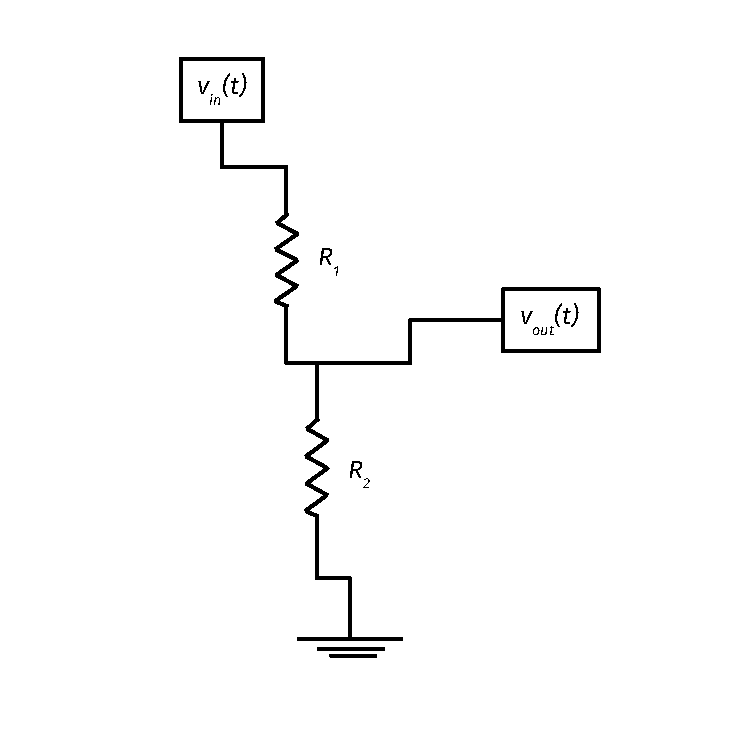
\includegraphics[width=0.5\textwidth]{AnalogExample/VoltageDivider.pdf}
\caption{\label{fig:example1} A two-resistor voltage divider.}
\end{figure}
\end{frame}

\begin{frame}{Analog and Digital}
\begin{itemize}
\item Using Ohm's Law, find expressions for $v_{\rm in}(t)$ and $v_{\rm out}(t)$ in terms of the resistances and the current.
\item Take the ratio of the output voltage to the input voltage to find the \textbf{transfer function}, $H(t)$.
\item Volunteer to board?
\end{itemize}
\end{frame}

\begin{frame}{Analog and Digital}
Answer:
\begin{equation}
H(t) = \frac{R_2}{R_1+R_2}
\end{equation} \\
\vspace{0.5cm}
In other words, the circuit does not change the time-domain properties of the signal, just the \textit{amplitude}. \\ \vspace{0.5cm}
Can we replace a resistor with another component to \textit{filter} signals based on time-domain properties?
\end{frame}

\begin{frame}{Analog and Digital}
\begin{figure}
\centering
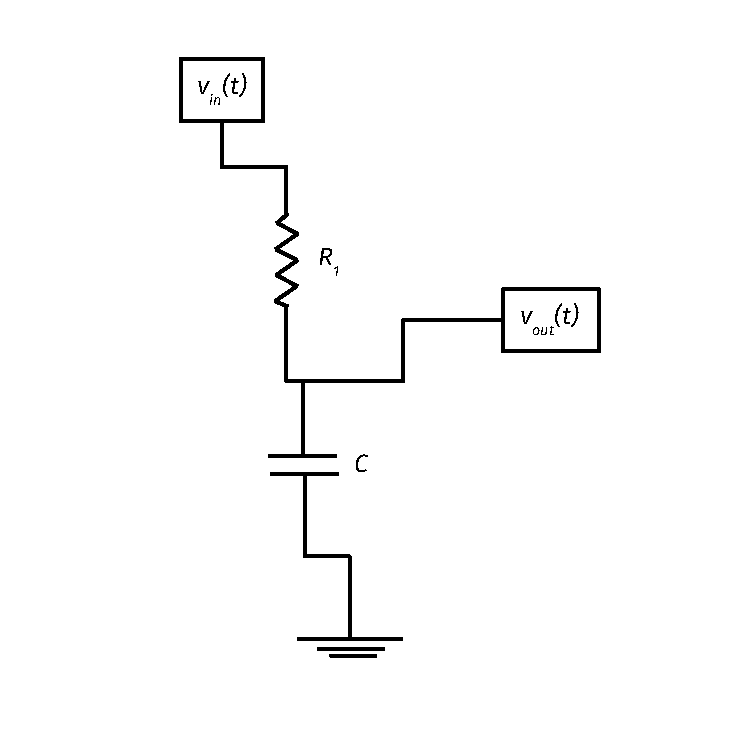
\includegraphics[width=0.5\textwidth]{AnalogExample/LowPass.pdf}
\caption{\label{fig:example2} A single-pole low-pass RC filter.  What is the resistance or impedance of a capacitor?}
\end{figure}
\end{frame}

\begin{frame}{Analog and Digital}
We need a math tool, the Fourier transform:
\begin{align}
\mathcal{F}(f(t)) = \tilde{F}(\omega) &= \int_{-\infty}^{\infty} f(t) e^{-j\omega t} dt \label{eq:eq1} \\
f(t) &= g'(t) \label{eq:eq2} \\
\tilde{F}(\omega) = g(t) e^{-j\omega t} |_{-\infty}^{\infty} + &j\omega \int_{\infty}^{-\infty} g(t)  e^{-j\omega t} dt \label{eq:eq3} \\
\mathcal{F}(g'(t)) &= j\omega\mathcal{F}(g(t)) \label{eq:eq4}
\end{align}
After integrating by parts we find that the Fourier transform of a derivative of a function is the imaginary unit times the angular frequency times the Fourier transform of the function.  \textbf{Note that throughout this course $j$ is the imaginary unit.  This is common in engineering texts.}
\end{frame}

\begin{frame}{Analog and Digital}
Impedance of a capacitor:
\begin{align}
C &= \frac{q}{V} \\
VC &= q \\
C \frac{dV}{dt} &= \frac{dq}{dt} = i(t) \\
\tilde{i}(\omega) &= j\omega C \tilde{V}(\omega) \\
\frac{\tilde{V}(\omega)}{\tilde{i}(\omega)} &= \frac{1}{j\omega C}
\end{align}
Using Ohm's Law, we identify the impedance as
\begin{equation}
\boxed{
Z_C = \frac{1}{j\omega C}
}
\label{eq:eq5}
\end{equation}
\end{frame}

\begin{frame}{Analog and Digital}
Repeat the earlier exercise, but with the new circuit:
\begin{itemize}
\item Using Ohm's Law, find expressions for $v_{\rm in}(t)$ and $v_{\rm out}(t)$ in terms of the impedances and the current.
\item Take the ratio of the output voltage to the input voltage to find the \textbf{transfer function}, $H(t)$.
\item Volunteer to board?
\end{itemize}
\end{frame}

\begin{frame}{Analog and Digital}
Answer:
\begin{equation}
\boxed{
M_{LP}(\omega) = \sqrt{\frac{\omega_0^2}{\omega^2+\omega_0^2}}
}
\label{eq:eq6}
\end{equation}

\begin{equation}
\boxed{
\phi_{LP}(\omega) = -\tan^{-1}\left(\frac{\omega}{\omega_0}\right)
}
\label{eq:eq7}
\end{equation} \\
\vspace{0.5cm}
The transfer function of this circuit depends on frequency in the following way:
\begin{enumerate}
\item $\omega \ll \omega_{\rm 0}$, $M_{\rm LP} \approx 1$, $\phi_{\rm LP} \approx 0$
\item $\omega \gg \omega_{\rm 0}$, $M_{\rm LP} \approx 0$, $\phi_{\rm LP} \approx -90^{\circ}$
\end{enumerate}
\end{frame}

\begin{frame}{Analog and Digital}
\begin{figure}
\centering
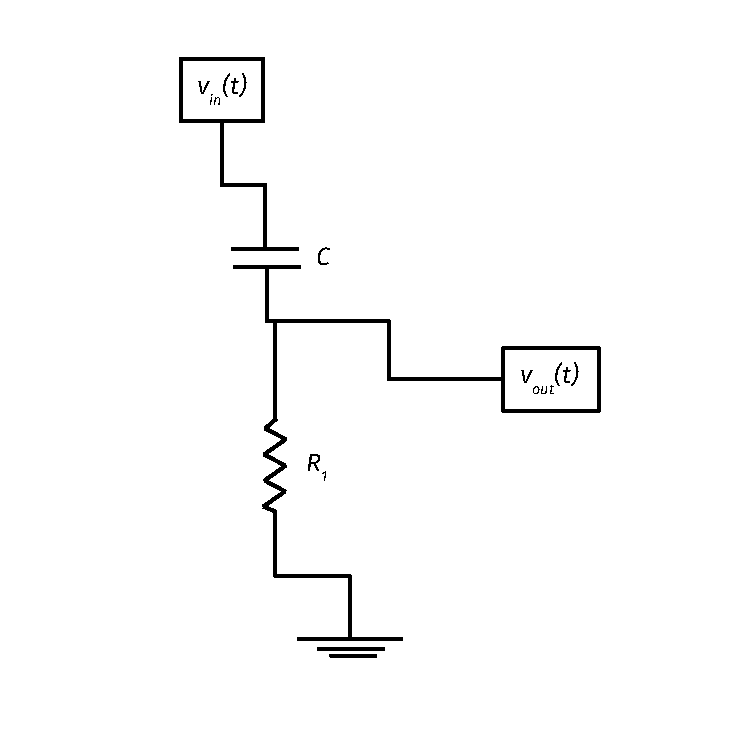
\includegraphics[width=0.5\textwidth]{AnalogExample/HighPass.pdf}
\caption{\label{fig:example3} A single-pole high-pass RC filter.  Can we repeat this process, only with the capacitor and resistor exchanged?}
\end{figure}
\end{frame}

\begin{frame}{Analog and Digital}
Answer:
\begin{equation}
\boxed{
M_{HP}(\omega) = \sqrt{\frac{\omega^2}{\omega^2+\omega_0^2}}
}
\label{eq:eq8}
\end{equation}

\begin{equation}
\boxed{
\phi_{HP}(\omega) = \tan^{-1}\left(\frac{\omega_0}{\omega}\right)
}
\label{eq:eq9}
\end{equation} \\
\vspace{0.5cm}
The transfer function of this circuit depends on frequency in the following way:
\begin{enumerate}
\item $\omega \ll \omega_{\rm 0}$, $M_{\rm HP} \approx 0$, $\phi_{\rm HP} \approx 90^{\circ}$
\item $\omega \gg \omega_{\rm 0}$, $M_{\rm HP} \approx 1$, $\phi_{\rm HP} \approx 0$
\end{enumerate}
\end{frame}

\begin{frame}{Analog and Digital}
\begin{figure}
\centering
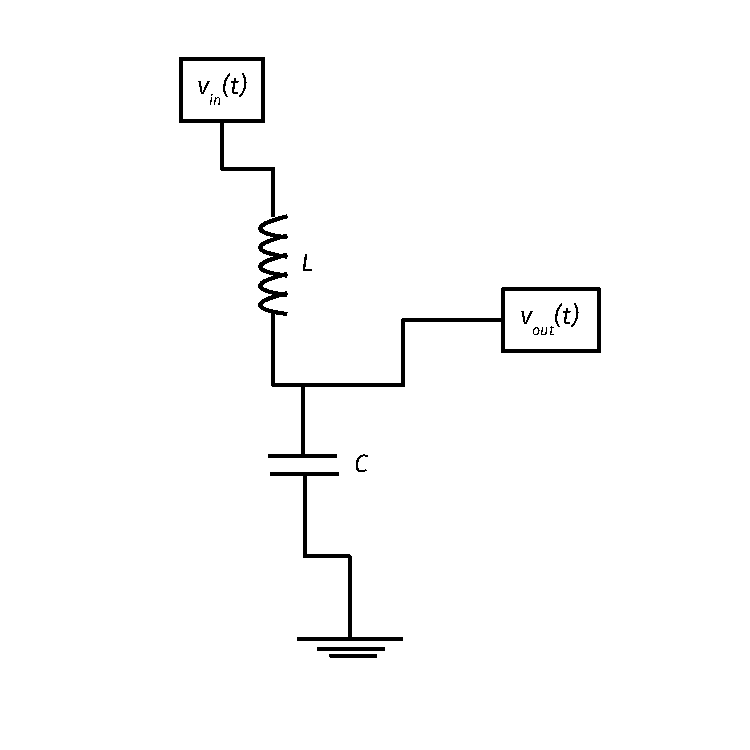
\includegraphics[width=0.5\textwidth]{AnalogExample/LowPassLC.pdf}
\caption{\label{fig:example4} A simple LC-resonator (two-pole).  What is the impedance of an inductor?}
\end{figure}
\end{frame}

\begin{frame}{Analog and Digital}
Impedance of an inductor:
\begin{align}
L &= \frac{d\phi}{di} \\
L &= \frac{d\phi}{dt}\frac{dt}{di} = v/i(t) \\
\tilde{v}(\omega) &= j\omega L\tilde{i}(\omega)
\end{align}
So we can read off the impedance of the inductor:
\begin{equation}
\boxed{
Z_{\rm L} = j\omega L}
\end{equation}
\end{frame}

\begin{frame}{Analog and Digital}
Following the same model, but with new impedances, we find Eq. \ref{eq:eq8} below by defining a \textit{resonance frequency} $\omega_R^{-2} = LC$. 
\begin{equation}
\boxed{
M_{\rm LC}(\omega) = \frac{\omega_R^2}{\omega_R^2-\omega^2} = \frac{\omega_R^2}{(\omega_R-\omega)(\omega_R + \omega)}
}
\label{eq:eq10}
\end{equation}
\end{frame}

\begin{frame}{Analog and Digital}
\tiny
\begin{columns}[T]
\begin{column}{0.5\textwidth}
\centering
\textbf{Analog circuits}
\begin{itemize}
\item Continuous functions of voltage and current representing continuous data
\item Application of complex analysis
\end{itemize}
\hrulefill
\begin{itemize}
\item Cannot be stored, copied or transmitted quickly and efficiently
\item Requires knowledge of every frequency (bandwidth issues)
\item Cannot be transmitted easily (noise issues)
\end{itemize}
\end{column}
\begin{column}{0.5\textwidth}
\centering
\textbf{Digital circuits}
\begin{itemize}
\item Discrete functions of voltage and current representing coded data
\item Application of Boolean logic
\end{itemize}
\hrulefill
\begin{itemize}
\item Must sample enough information to reproduce analog signals
\end{itemize}
\end{column}
\end{columns}
Music is an obvious example: storiing music on a vinyl record creates a groove in the material of the record that follows the pressure wave pattern of the sound.  At no point are any frequencies lost, unless the record is scratched.  When music is stored digitally, the sample rate affects quality, but with a large sample rate, the music is indistinguishable from the record player.  Plus, the music can be perfectly copied or transmitted.
\end{frame}

\section{Introduction to Digital Concepts}

\begin{frame}{Introduction to Digital Concepts}
Recall from the low and high pass filter examples:
\begin{enumerate}
\item $\omega \ll \omega_{\rm 0}$, $M_{\rm HP} \approx 0$, $\phi_{\rm HP} \approx 90^{\circ}$
\item $\omega \gg \omega_{\rm 0}$, $M_{\rm HP} \approx 1$, $\phi_{\rm HP} \approx 0$
\end{enumerate}
\hrulefill
\begin{enumerate}
\item $\omega \ll \omega_{\rm 0}$, $M_{\rm LP} \approx 1$, $\phi_{\rm LP} \approx 0$
\item $\omega \gg \omega_{\rm 0}$, $M_{\rm LP} \approx 0$, $\phi_{\rm LP} \approx -90^{\circ}$
\end{enumerate}
What if instead of a frequency-based filter, we had an amplitude-based filter? (Also known as transistors...stay tuned).
\end{frame}

\begin{frame}{Introduction to Digital Concepts}
\begin{figure}
\centering
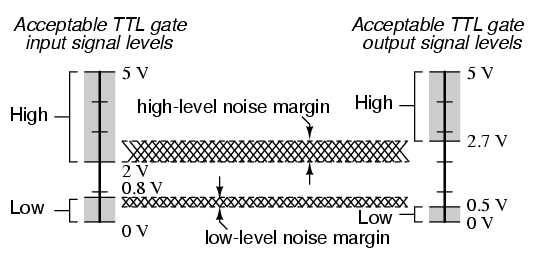
\includegraphics[width=0.7\textwidth]{figures/TTL.png} \hspace{0.1cm}
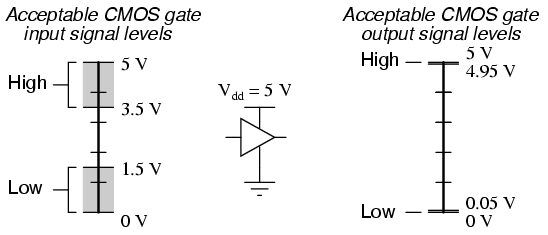
\includegraphics[width=0.7\textwidth]{figures/CMOS.png}
\caption{\label{fig:levels} TTL and CMOS logic levels in integrated circuits today.}
\end{figure}
\end{frame}

\begin{frame}{Introduction to Digital Concepts}
\begin{figure}
\centering
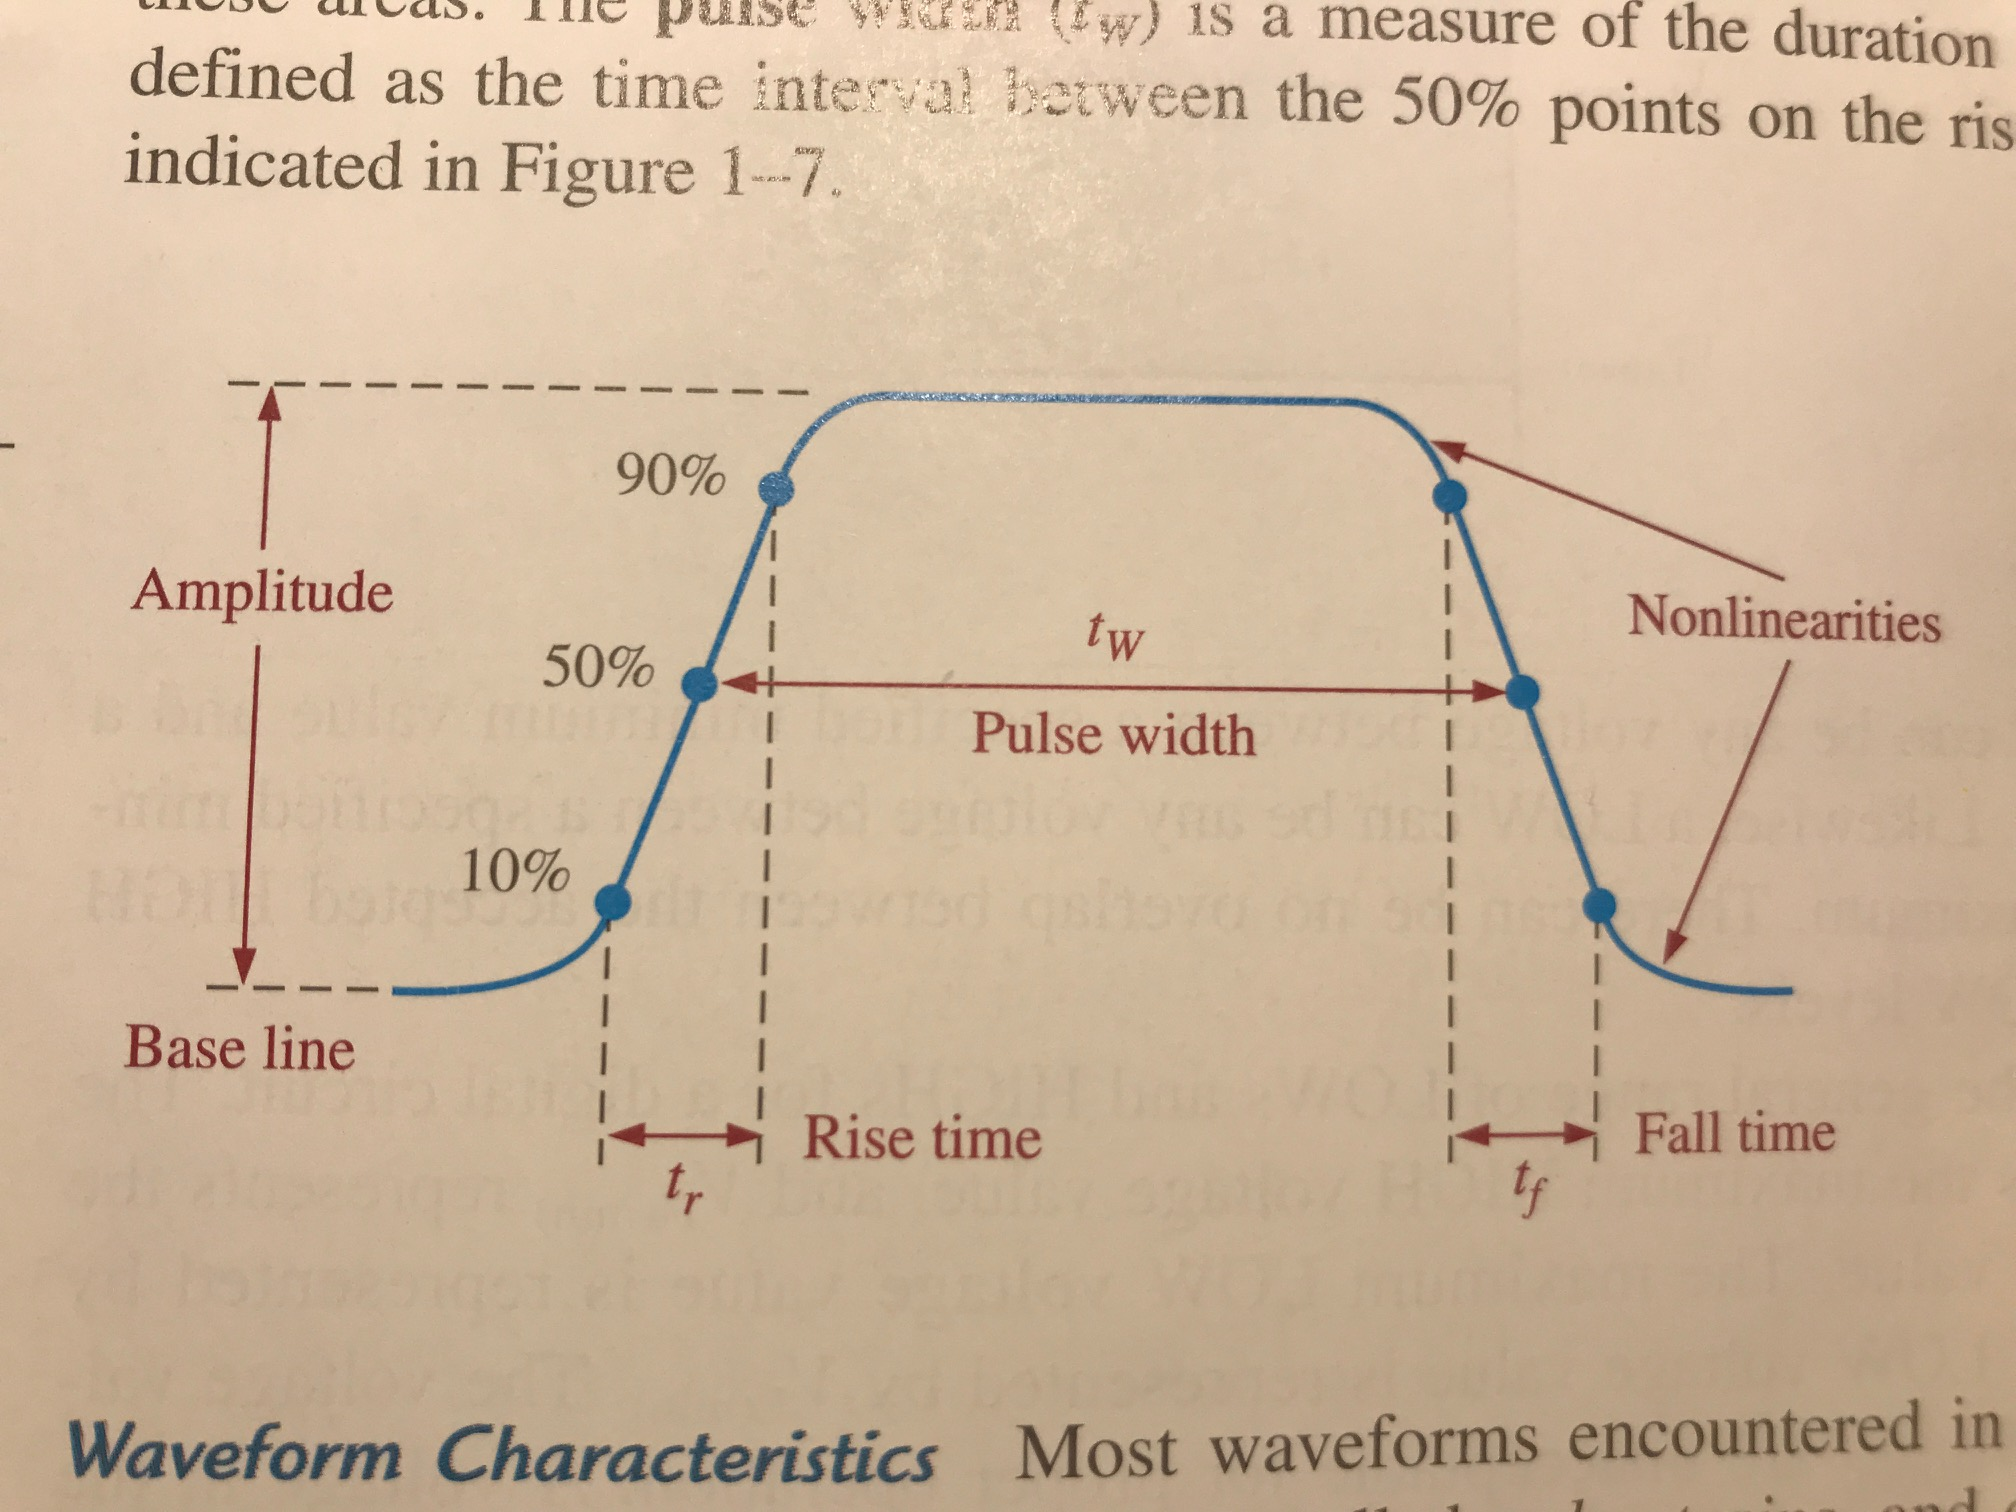
\includegraphics[width=0.5\textwidth,trim=1cm 7cm 0cm 9cm,clip=true]{figures/pulse.jpg}
\caption{\label{fig:pulse} Properties of the logic pulse: rise and fall times, amplitude and non-linearities.}
\end{figure}
From where do the non-linearities arise? Turns out the Fourier transform of a square wave $s(t)$ with period $T$ is a ``sync'' function $(2\pi\nu = \omega)$:
\begin{equation}
\mathcal{F}(s(t)) = \tilde{S}(\nu) = \frac{\sin(\pi\nu T)}{\pi\nu}
\end{equation}
\end{frame}

\begin{frame}{Introduction to Digital Concepts}
From where do the non-linearities arise? Turns out the Fourier transform of a square wave $s(t)$ with period $T$ is a ``sync'' function $(2\pi\nu = \omega)$:
\begin{equation}
\mathcal{F}(s(t)) = \tilde{S}(\nu) = \frac{\sin(\pi\nu T)}{\pi\nu}
\end{equation}
The \textbf{convolution theorem} states that if a signal is being filtered, the transfer function of that filter is being multiplied with the Fourier transform of the signal in the Fourier domain.  Let's \textit{low-pass filter} the sync function:
\begin{align}
\tilde{S}(\nu)H_{\rm LP}(\omega) &= \frac{\sin(\pi\nu T)}{\pi\nu}\sqrt{\frac{\omega_0^2}{\omega^2+\omega_0^2}} \\
\tilde{S}(\nu)H_{\rm LP}(\omega) &= \frac{\sin(\pi\nu T)}{\pi\nu(1+(2\pi\nu\tau)^2)^{1/2}}, \tau = \omega_{\rm 0}^{-1}
\end{align}
\end{frame}

\begin{frame}{Introduction to Digital Concepts}
\begin{figure}
\centering
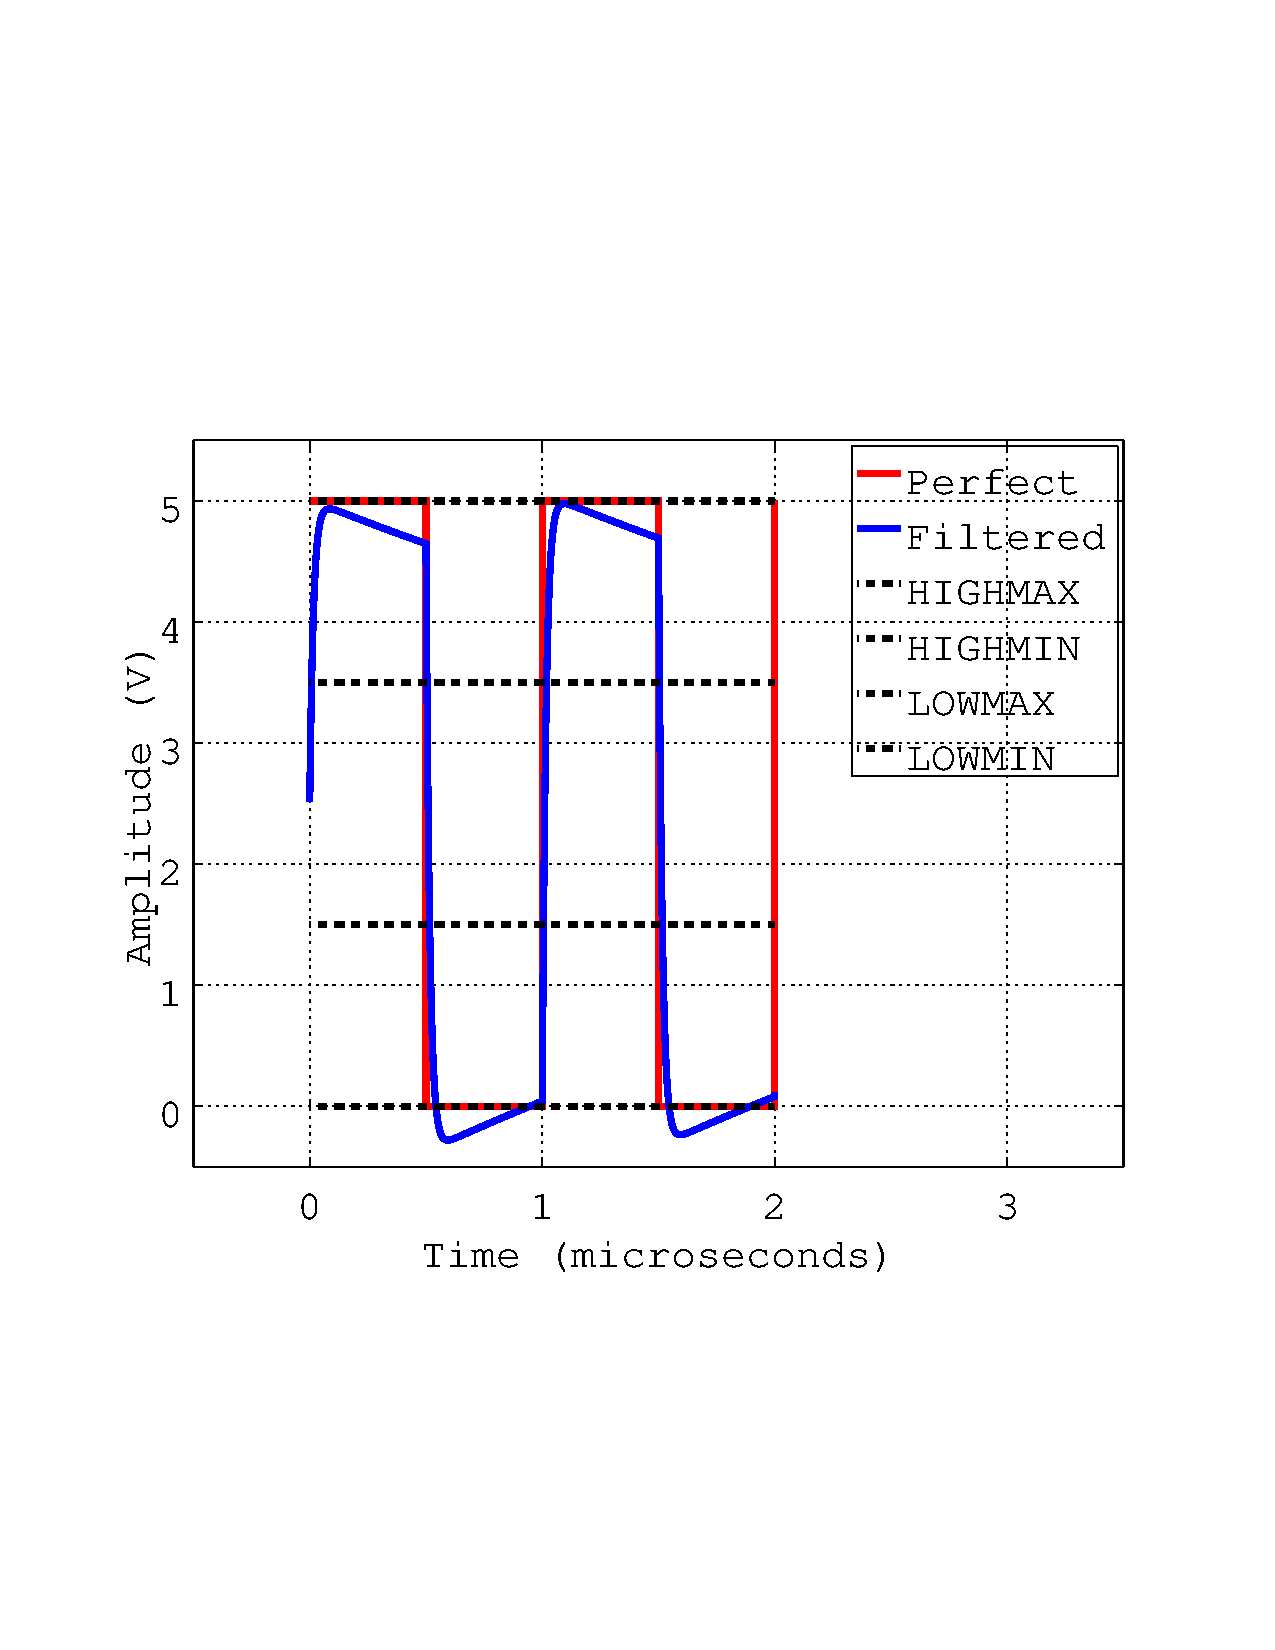
\includegraphics[width=0.75\textwidth,trim=1cm 6cm 1cm 7cm,clip=true]{codes/January8_plot1.pdf}
\caption{\label{fig:pulse2} CMOS logic pulse filtered to remove frequencies above 0.01 MHz and below 2 MHz for a 1 MHz clock frequency.}
\end{figure}
\end{frame}

\begin{frame}{Introduction to Digital Concepts}
\alert{\textbf{Fourier transform}}:
\begin{equation}
\mathcal{F}(f(t)) = \int_{-\infty}^{\infty} f(t) \exp(-2\pi j\nu t) dt
\end{equation}
\textbf{In-class exercises}.  Evaluate the Fourier transform of each of the following functions/distributions:
\begin{enumerate}
\item $f(t) = \delta(t-t_{\rm 0})$
\item $f(t) = \exp(-at)$, for $t>=0$, $0$ for $t<0$
\end{enumerate}
Now compute the modulus-squared for each result: $z^{*}z = |z|^2$.  What is the frequency-dependence of each?
\end{frame}

\begin{frame}{Introduction to Digital Concepts}
\small
Pulse-waveform vocabulary:
\begin{enumerate}
\item \textbf{Period} - Time required for a repeating signal to return to original state.
\item \textbf{Frequency} - Inverse of the period.
\item \textbf{Pulse width} - Width of time between identical signal values
\item \textbf{Rise time} - Time required for the signal to rise from 10\% to 90\% of the amplitude
\item \textbf{Fall time} - Similar to fall time but for amplitude decrease
\item \textbf{Duty cycle} - Pulse width divided by period
\end{enumerate}
\end{frame}

\begin{frame}{Introduction to Digital Concepts}
\textbf{Major feature of digital circuit components}: \textit{any} voltage between HIGHMAX and HIGHMIN is HIGH, and \textit{any} voltage between LOWMAX and LOWMIN is LOW.  Issues of bandwidth and filtering are nullified because the circuit will perform the correct action \textit{regardless of these effects.} \\
\begin{table}
\centering
\begin{tabular}{c | c}
HIGH & 1 \\ \hline
LOW & 0 \\
\end{tabular}
\caption{\label{tab:highlow} Digital circuits strategically neglect the analog nature of the voltage inputs.}
\end{table}
\end{frame}

\begin{frame}{Introduction to Digital Concepts}
\begin{figure}
\centering
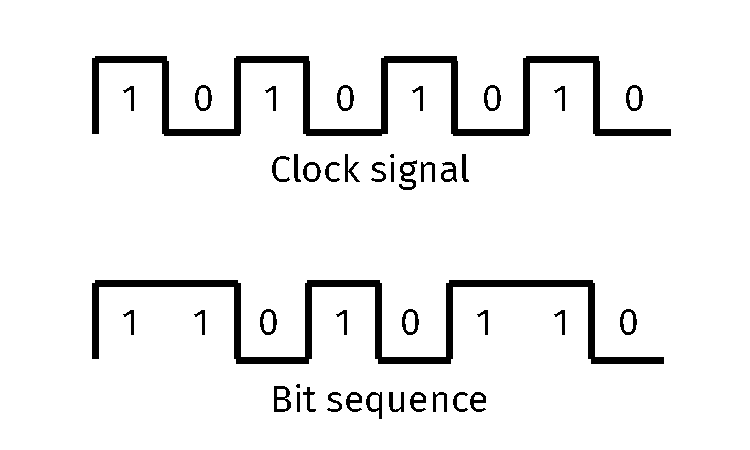
\includegraphics[width=0.75\textwidth]{figures/BitSequence.pdf}
\caption{\label{fig:bitsequence} The clock simply switches between HIGH and LOW periodically.  Normal data sequences are strings of \textit{bits}.  In this case, we have 11010110.}
\end{figure}
\end{frame}

\begin{frame}{Introduction to Digital Concepts}
\begin{figure}
\centering
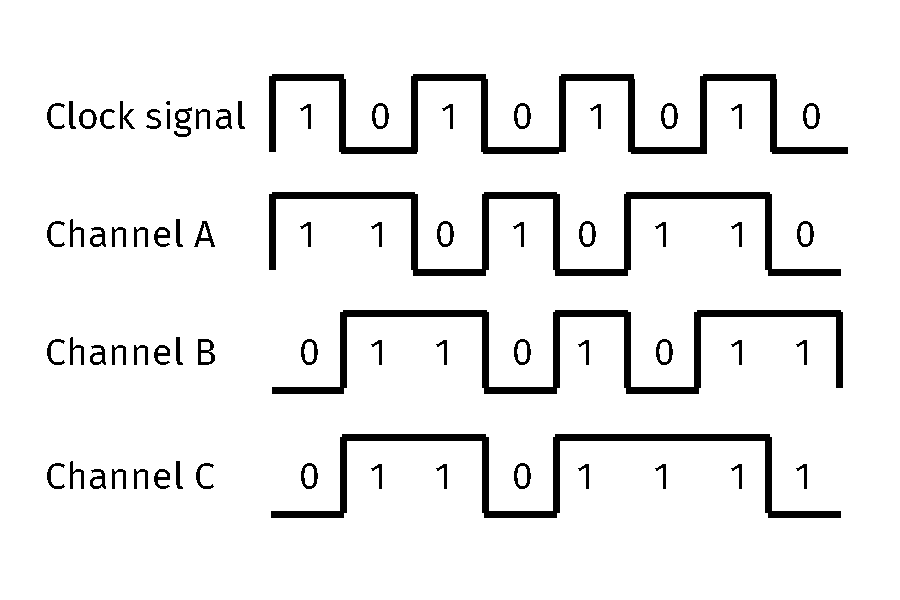
\includegraphics[width=0.75\textwidth]{figures/BitSequence2.pdf}
\caption{\label{fig:bitsequence2} A timing diagram.  A display of the synchronized bit sequences of multiple data channels.}
\end{figure}
\end{frame}

\begin{frame}{Introduction to Digital Concepts}
\begin{figure}
\centering
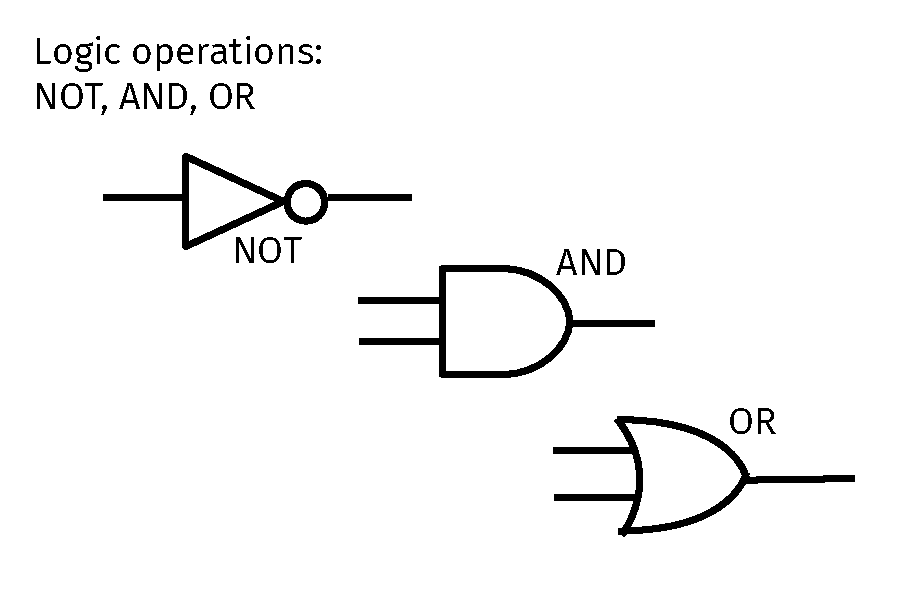
\includegraphics[width=0.75\textwidth]{figures/Operators.pdf}
\caption{\label{fig:operators} Bit sequences can be inputs to \textbf{logic operations}, performed by \textit{gates} (more later).}
\end{figure}
\end{frame}

\begin{frame}{Introduction to Digital Concepts}
\begin{columns}[T]
\begin{column}{0.5\textwidth}
\begin{table}
\centering
\begin{tabular}{c | c}
Input & Output \\ \hline
1 & 0 \\ \hline
0 & 1 \\
\end{tabular}
\caption{\label{tab:not} NOT truth table.}
\end{table}
\begin{table}
\centering
\begin{tabular}{c | c | c}
Input1 & Input2 & Output \\ \hline
1 & 1 & 1 \\ \hline
1 & 0 & 0 \\ \hline
0 & 1 & 0 \\ \hline
0 & 0 & 0 \\ \hline
\end{tabular}
\caption{\label{tab:and} AND truth table.}
\end{table}
\end{column}
\begin{column}{0.5\textwidth}
\begin{table}
\centering
\begin{tabular}{c | c | c}
Input1 & Input2 & Output \\ \hline
1 & 1 & 1 \\ \hline
1 & 0 & 1 \\ \hline
0 & 1 & 1 \\ \hline
0 & 0 & 0 \\ \hline
\end{tabular}
\caption{\label{tab:or} OR truth table.}
\end{table}
\end{column}
\end{columns}
\end{frame}

\begin{frame}{Introduction to Digital Concepts}
\small
\begin{figure}
\centering
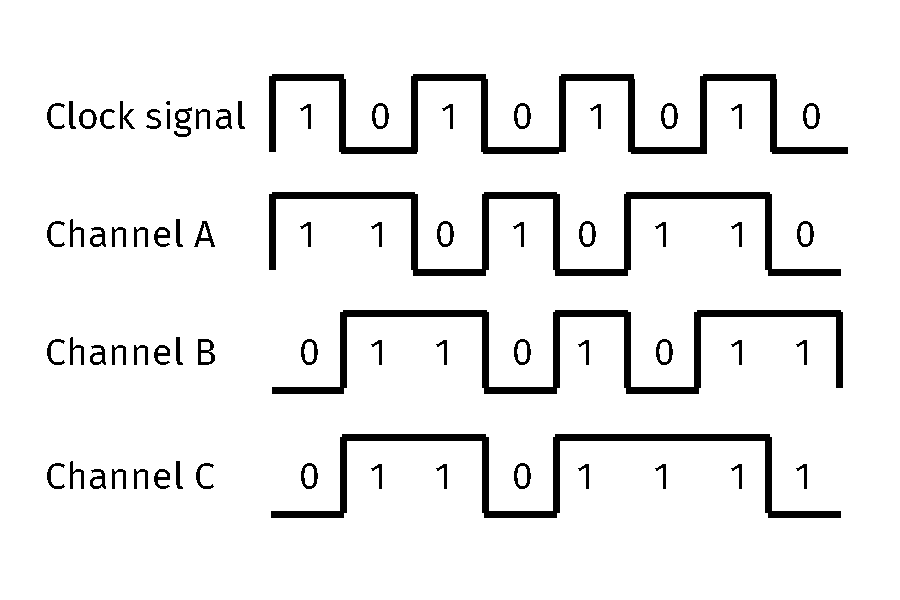
\includegraphics[width=0.4\textwidth]{figures/BitSequence2.pdf}
\caption{\label{fig:bitsequence3} Bit sequences $\rightarrow$ logic operations $\rightarrow$ new bit sequences.}
\end{figure}
Write down the following bit sequences:
\begin{enumerate}
\item NOT A
\item A OR Clock
\item A AND B
\item A AND (B OR C)
\end{enumerate}
\end{frame}

\begin{frame}{Introduction to Digital Concepts}
\small
Volunteers to board?
\begin{enumerate}
\item NOT A
\item A OR Clock
\item A AND B
\item A AND (B OR C)
\end{enumerate}
How would you express the final exercise in terms of gates representing logic operations and bit sequences as inputs?
\end{frame}

\begin{frame}{Introduction to Digital Concepts}
\small
\begin{figure}
\centering
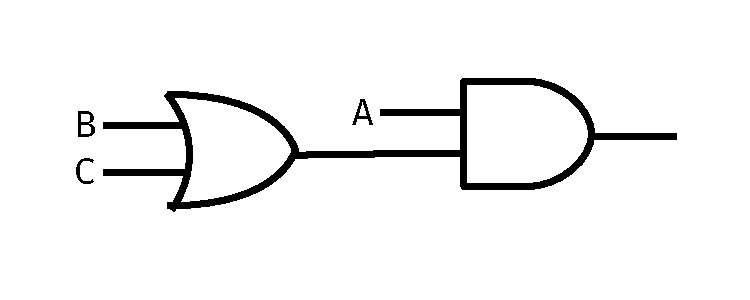
\includegraphics[width=0.7\textwidth]{figures/Operators2.pdf}
\caption{\label{fig:bitsequence4} Solution: do the grouping symbol first, as in order of operations.}
\end{figure}
\end{frame}

\begin{frame}{Introduction to Digital Concepts}
Compose a circuit of gates that produces the following bit sequences:
\begin{enumerate}
\item (NOT (A AND B)) OR C
\item NOT A AND B
\item A AND B AND C AND D
\item (A OR B) AND (A OR B)
\end{enumerate}
\end{frame}

\begin{frame}{Introduction to Digital Concepts}
\begin{columns}[T]
\begin{column}{0.5\textwidth}
A few more logic operators:
\begin{enumerate}
\item \textbf{\alert{Comparator}}
\item Adder
\item Encoder
\item Decoder
\item Shift register
\item Flip-flop
\item Multiplexer
\item Demultiplexer
\item Counter
\end{enumerate}
\end{column}
\begin{column}{0.5\textwidth}
\begin{figure}
\centering
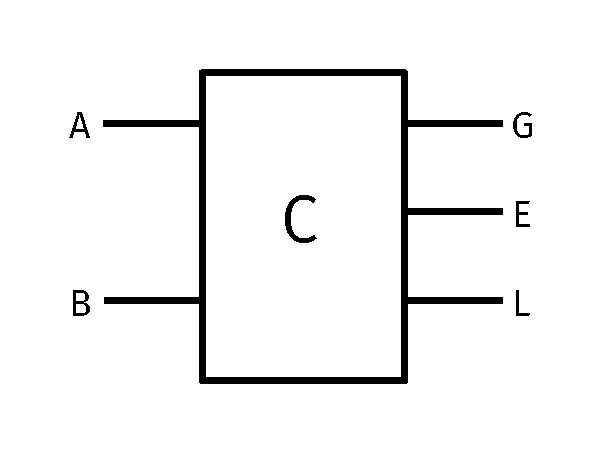
\includegraphics[width=0.9\textwidth]{figures/Comparator.pdf}
\caption{\label{fig:comparator} A comparator compares bit sequences A and B, and raises G to HIGH if A represents a number greater than B, E if they are equal, and L if A is less than B.}
\end{figure}
\end{column}
\end{columns}
\end{frame}

\begin{frame}{Introduction to Digital Concepts}
\begin{columns}[T]
\begin{column}{0.5\textwidth}
A few more logic operators:
\begin{enumerate}
\item Comparator
\item \textbf{\alert{Adder}}
\item Encoder
\item Decoder
\item Shift register
\item Flip-flop
\item Multiplexer
\item Demultiplexer
\item Counter
\end{enumerate}
\end{column}
\begin{column}{0.5\textwidth}
\begin{figure}
\centering
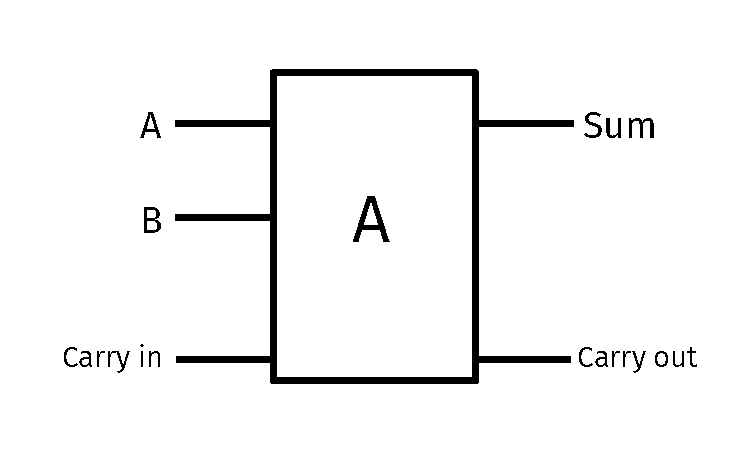
\includegraphics[width=\textwidth]{figures/Adder.pdf}
\caption{\label{fig:adder} An adder adds two binary numbers (bit sequences A and B here) in the same way we add numbers on paper.  We \textit{carry} powers of 10 (2) on paper (in binary).}
\end{figure}
\end{column}
\end{columns}
\end{frame}

\begin{frame}{Introduction to Digital Concepts}
\textbf{Group board exercise}:
Compose a circuit that records adds two inputs, compares the result to a third input, and has an output of HIGH if the sum of the first two inputs is greater than the third input.  \textit{Use more than one adder, but assume that the numbers are small enough to not need the last $C_{\rm out}$}.
\end{frame}

\begin{frame}{Introduction to Digital Concepts}
But wait, how can the adder physically know how to add if it receives the digits one by one?  Don't all these elements operate on clock cycles? \\ \vspace{0.5cm}
Good question.  We need the concept of \textit{serial data} versus \textit{parallel data}. \\ \vspace{0.5cm}
\begin{itemize}
\item \textbf{Serial data}: one connection, many clock cycles per bit sequence.
\item \textbf{Parallel data}: many connections, one clock cycle per bit sequence.
\end{itemize}
\end{frame}

\begin{frame}{Introduction to Digital Concepts}
\begin{columns}[T]
\begin{column}{0.5\textwidth}
A few more logic operators:
\begin{enumerate}
\item Comparator
\item Adder
\item \textbf{\alert{Encoder}}
\item Decoder
\item Shift register
\item Flip-flop
\item Multiplexer
\item Demultiplexer
\item Counter
\end{enumerate}
\end{column}
\begin{column}{0.5\textwidth}
\begin{figure}
\centering
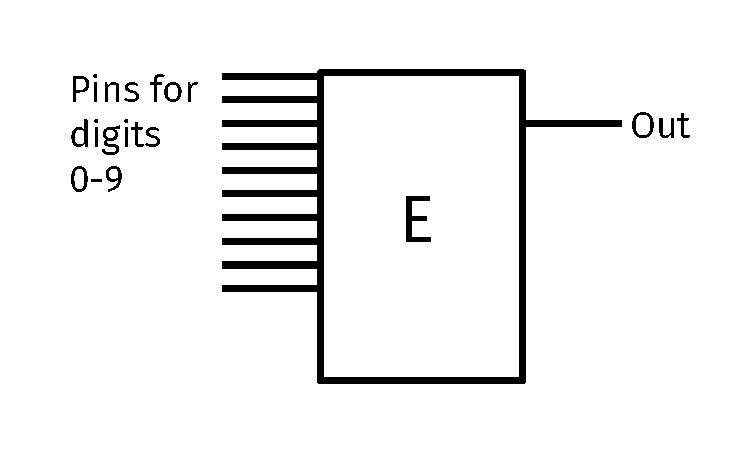
\includegraphics[width=\textwidth]{figures/Encoder.pdf}
\caption{\label{fig:encoder} The encoder has preset pins corresponding to (for example) digits 0-9, and the output bit sequence is a binary representation of the input that is raised HIGH.}
\end{figure}
\end{column}
\end{columns}
\end{frame}

\begin{frame}{Introduction to Digital Concepts}
\textbf{Group board exercise - final battle}:
Compose a circuit that takes as inputs two numbers 0-9, and adds them.  The output of the circuit is HIGH if and only if the result is between 8 and 12, inclusive.
\end{frame}

\section{Lab Tour, and Introduction to Lab Project 1}

\begin{frame}{Lab Tour, and Introduction to Lab Project 1}
\small
\begin{columns}[T]
\begin{column}{0.5\textwidth}
Our first project is an AM transistor radio (pictured at right). Goals:
\begin{itemize}
\item Share the experience of \alert{diving into an electronics project} blind
\item Understand why transistors revolutionized this device
\item Learn how a transistor works
\item Learn how to use test equipment like DVMs
\item Learn how to solder
\end{itemize}
\end{column}
\begin{column}{0.5\textwidth}
\begin{figure}
\centering
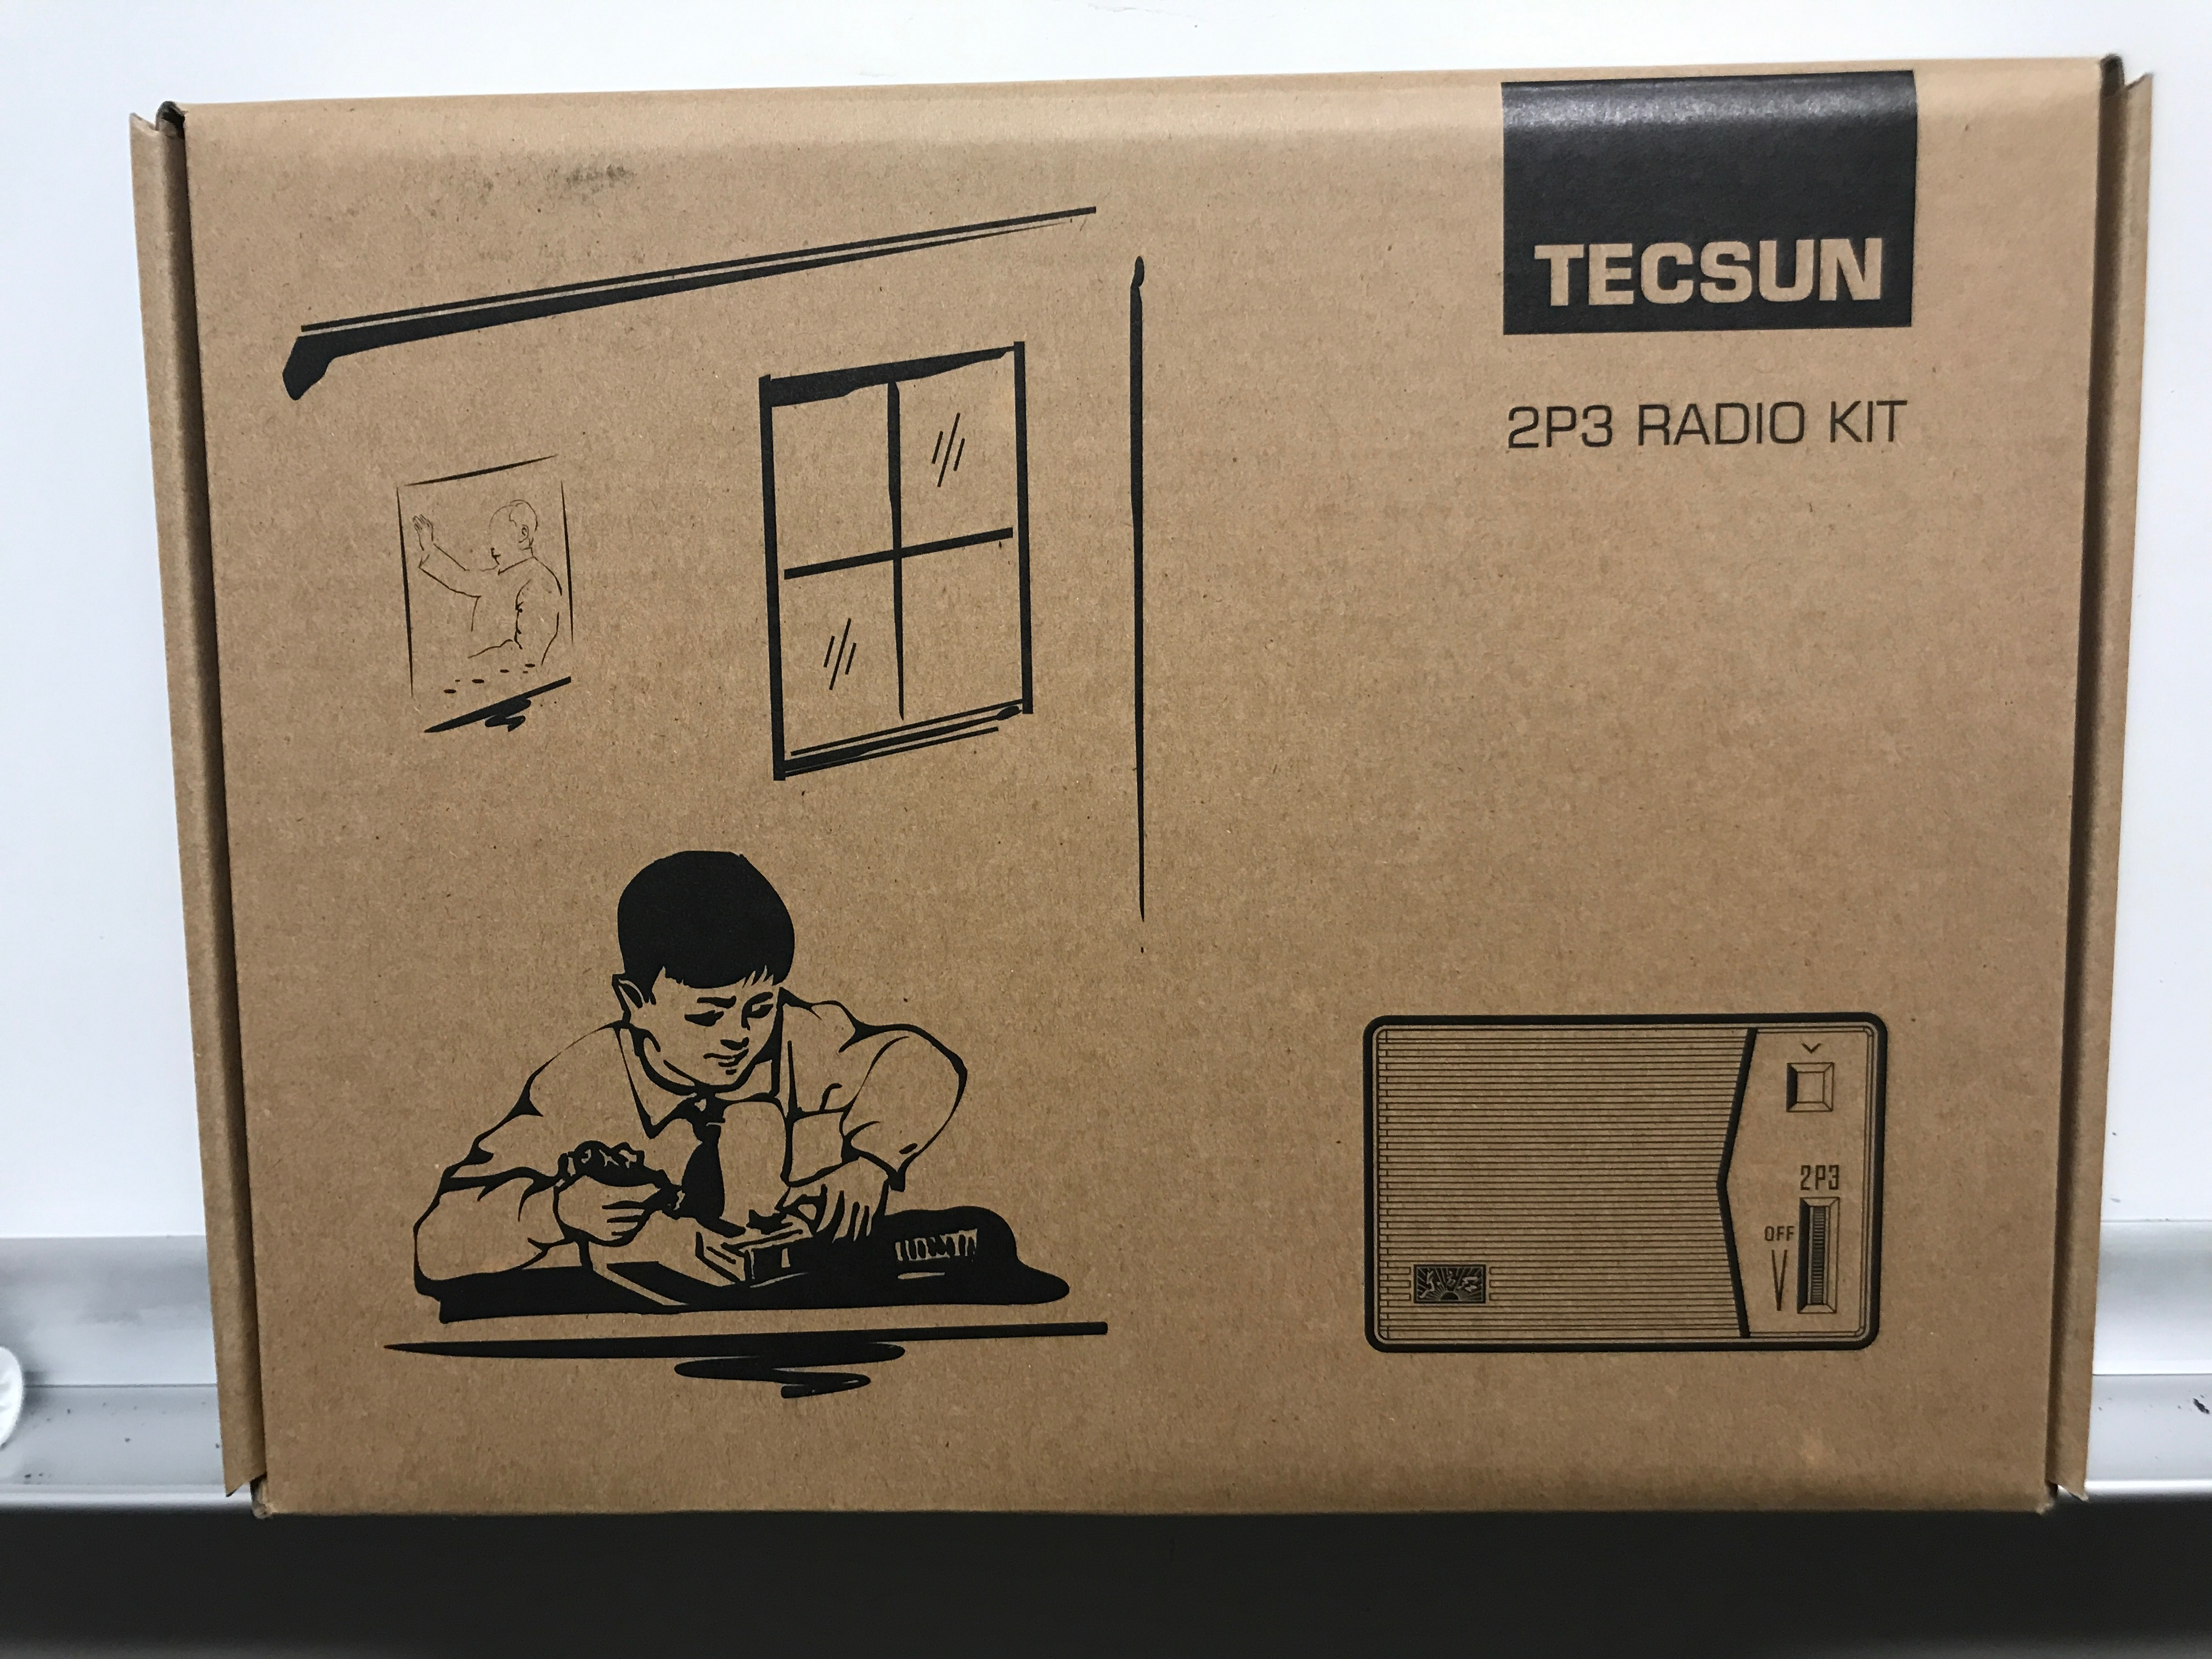
\includegraphics[width=0.9\textwidth]{figures/Tecsun.jpeg}
\caption{\label{fig:tec} The TecSun 2P3 transitor radio.}
\end{figure}
\end{column}
\end{columns}
\end{frame}

\section{Conclusion}

\begin{frame}{Unit 0 Summary - Introduction to Digital Concepts}
\textbf{Reading: Digital Fundamentals (DF) Ch. 1 (see Moodle)}
\begin{enumerate}
\item Analog and Digital - RC filters and LC resonators
\item Introduction to digital concepts
\item Transistor radio...go!
\end{enumerate}
\textbf{Homework: exercises 1-20 Ch. 1 (DF)}
\end{frame}

\end{document}
